\section{Modeling Coral Reef Dynamics}

\begin{frame}
\frametitle{Coral Reef Dynamics}
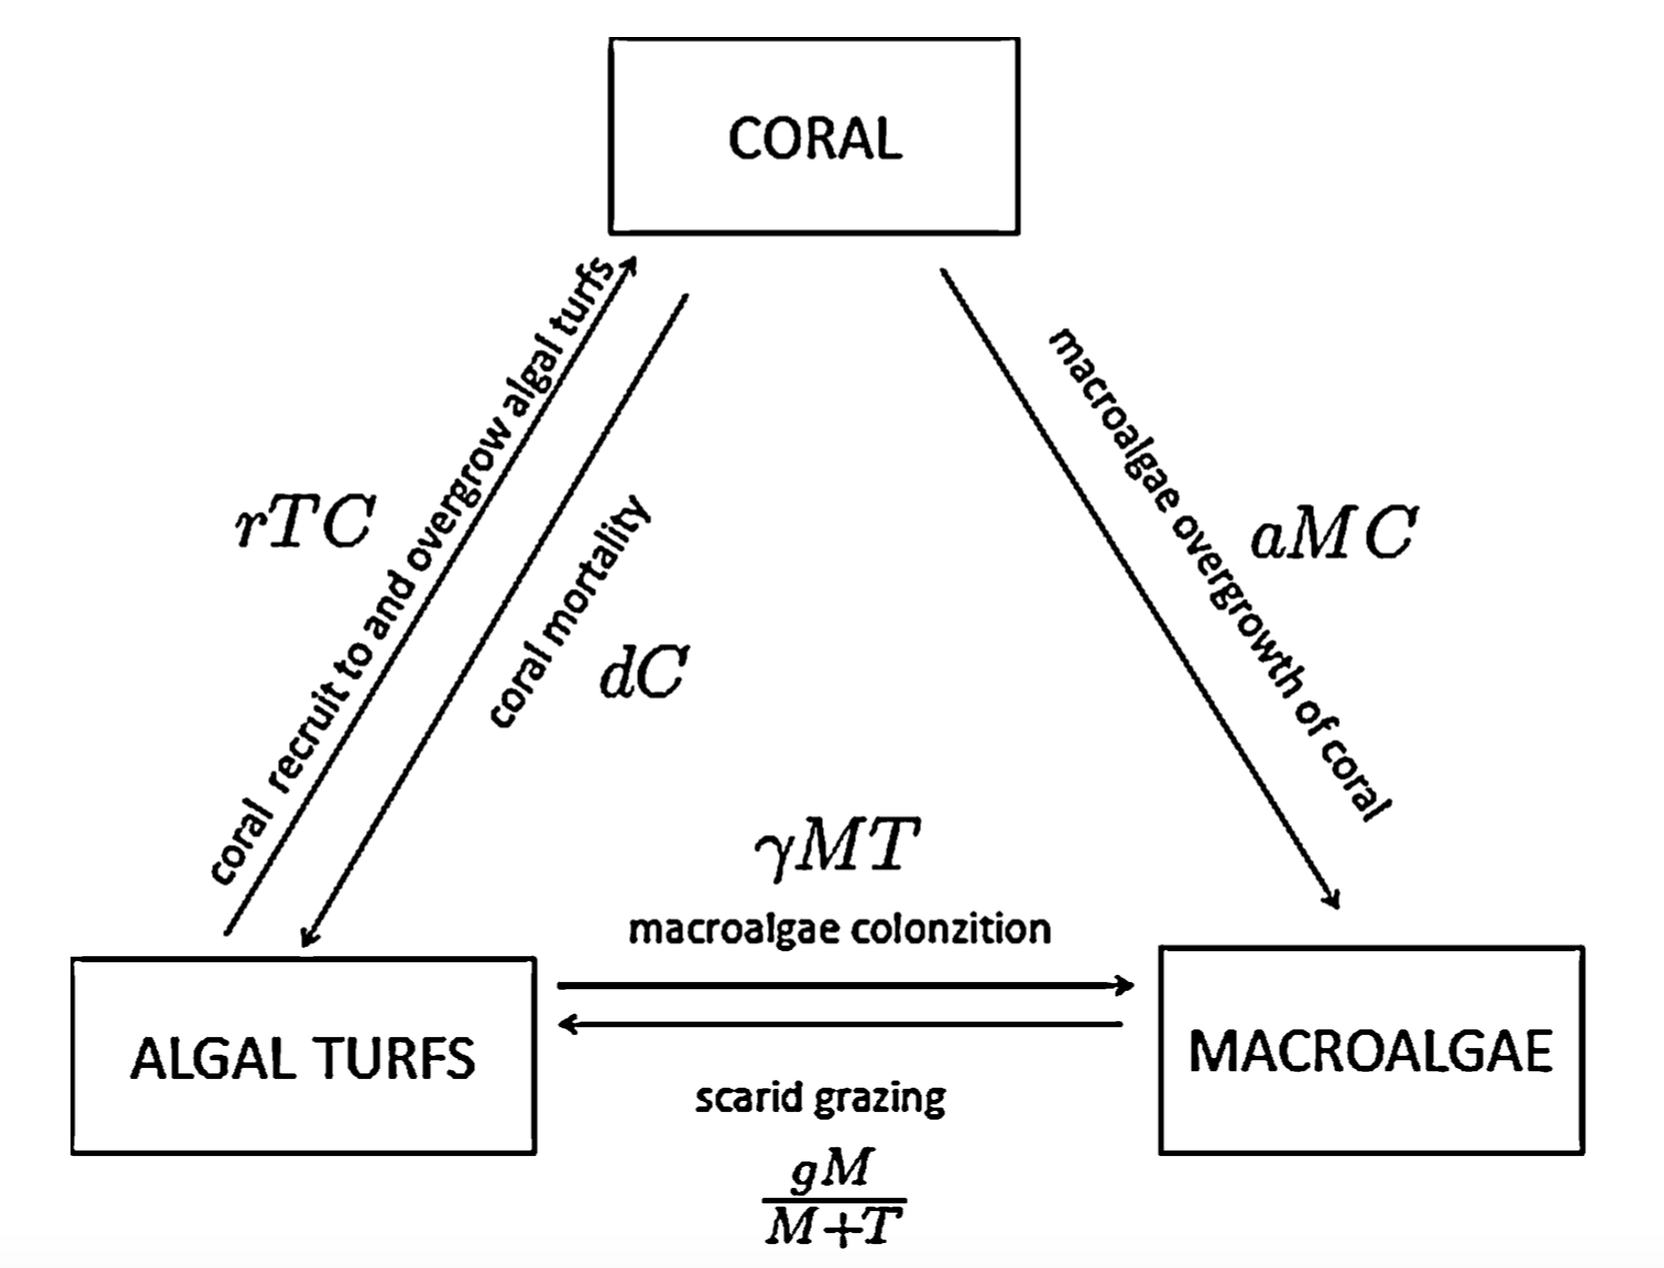
\includegraphics[scale=.175]{./coral-reef-triangle.png}\\ \cite{Hastings}
\end{frame}

\begin{frame}\frametitle{Coral Reef Dynamics}
The deterministic ordinary differential equation model:
$$\begin{cases}\begin{array}{rl}
\frac{dM}{dt}\hspace{-.8em}&=aMC - \frac{gM}{M+T} + \gamma M T, \\
\frac{dC}{dt}\hspace{-.8em}&=rTC - dC - aMC, \\
\frac{dT}{dt}\hspace{-.8em}&=\frac{gM}{M + T} - \gamma MT - rTC + dC. 
\end{array}\end{cases}$$ 

where 
\begin{itemize}\itemsep0pt
\item $r$ is the rate corals overgrow upon algal turfs\\
\item $d$ is the mortality rate of corals\\
\item $a$ is the rate that macroalgae overgrow upon corals\\
\item $\gamma$ is the rate that macroalgae spread over algal turfs\\
\item $g$ is the indiscriminate grazing rate of scarid
\end{itemize} We also assume $a<d<\gamma<r<2\gamma$ and $0<g<\gamma$. \vspace{1em}
\cite{Hastings}
\end{frame}

\begin{frame}\frametitle{Coral Reef Dynamics}

\hspace{1.57em}

\begin{itemize}
\item $\frac{dT}{dt}=-\frac{dM}{dt}-\frac{dC}{dt}$ implies $M+C+T$ is
  constant.
\item We assume that $M+C+T=1$.
\item This limits our scope to regions entirely covered by coral,
  macroalgae, and algal turf. 
\end{itemize}

Thus, we reduce our system to, 
$$\begin{cases}
\begin{array}{rl}
\frac{dM}{dt}&= aMC-\frac{gM}{1-C} + \gamma M - \gamma M^2 -\gamma M C,\\
\frac{dC}{dt}&=rC - rC^2 - rCM - dC - aMC.
\end{array} 
\end{cases}$$
\end{frame}


\begin{comment}\frametitle{Equilibria and Stability}
Equilibrium point

\end{comment}

\begin{frame}\frametitle{Equilibria and Stability}
To find equilibrium points analytically we first set the derivatives equal to zero to obtain the nullclines:
$$\begin{cases}
\begin{array}{rl}
0\hspace{-.8em}&=M(aC + \gamma-\gamma M-\gamma C - \frac{g}{1-C}),\\
0\hspace{-.8em}&=C(r-Mr-Cr - d - aM).
\end{array}
\end{cases}$$
\end{frame}



\begin{frame}\frametitle{Equilibria and Stability}

  \begin{itemize}
  \item $M'=0$ is satisfied when:
    \begin{itemize}
    \item $M=0$, or 
    \item
      $aC + \gamma - \gamma M - \gamma C -
      \frac{g}{1-C}=0$.
    \end{itemize}
  \item $C'=0$ is satisfied when:
    \begin{itemize} 
    \item$C=0$, or 
    \item $r-Mr-Cr-d-aM=0$. 
    \end{itemize}
  \end{itemize}

\end{frame}


\begin{frame}\frametitle{Phase Plane} 

  %Our equilibrium points are located at the intersections of the nullclines:\\
  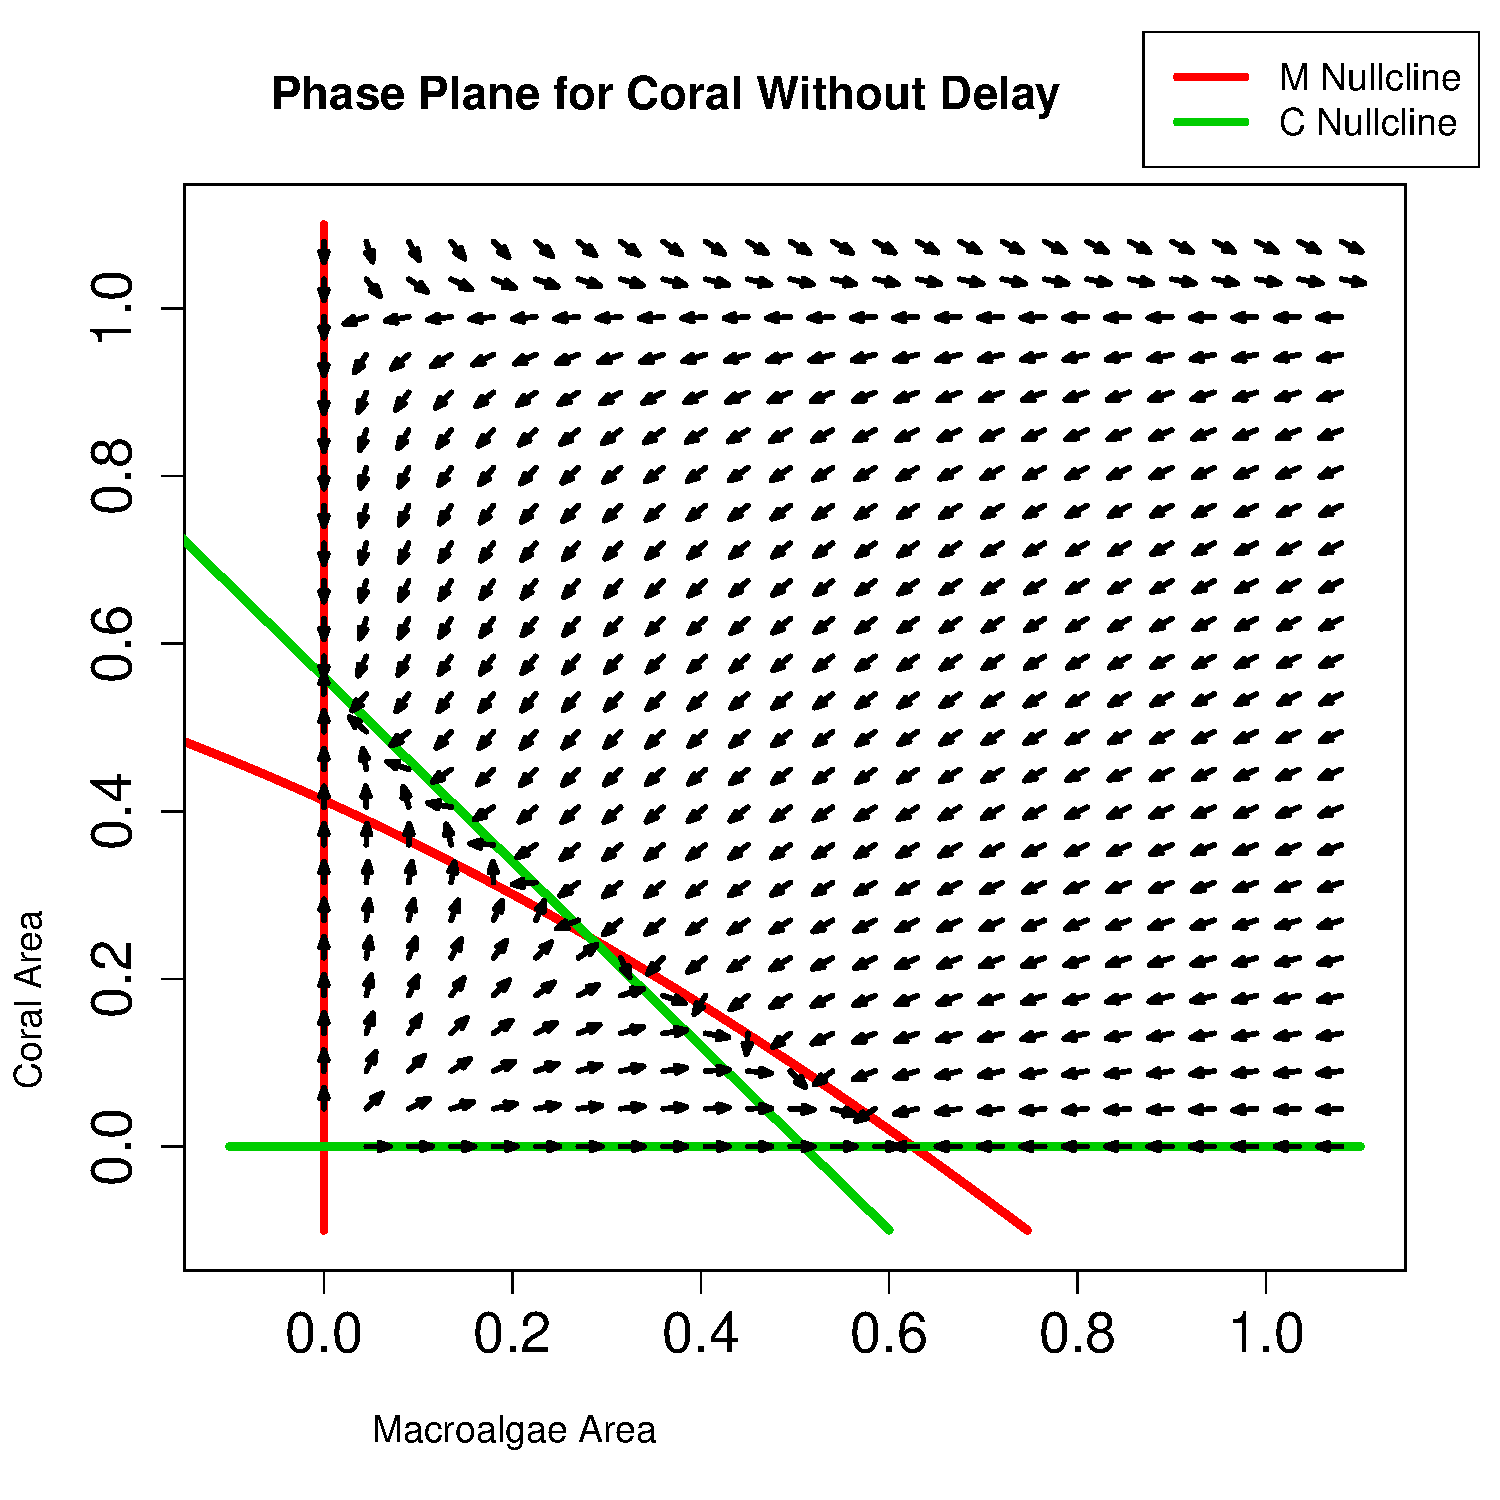
\includegraphics[scale=.325]{./nullclines.pdf}

\end{frame}



\begin{frame}
\frametitle{Time Delay in the Coral Ecosystem}

We can identify time delays in the coral ecosystem:
\begin{itemize}
\item the delay between overfishing of herbivores and growth of
  macroalgae \cite{Dinsdale},
\item the delay between the growth of algae and the effect of algae on
  coral, \cite{Mumby} 
\item the delay between the grazing of macroalgae and growth of algal
  turf \cite{Hastings}.
\end{itemize} We focus on the third phenomena.

\end{frame}


\begin{frame}\frametitle{Coral Reef Dynamics}
Scarid grazing has an impact for the macroalgae in the future:
$$\begin{cases}
  \begin{array}{rl}
    \frac{dM}{dt}\hspace{-.8em}&=aMC - \frac{gM(t-\tau)}{1-C(t-\tau)} + \gamma M (1-M-C),\\
    \frac{dC}{dt}\hspace{-.8em}&=rC(1-M-C) - dC - aMC,\\
  \end{array}
\end{cases}$$ where $\tau$ is a fixed time delay.
\end{frame}


\begin{frame}
\frametitle{Equilibria and Stability}
These are three equilibrium points of interest: 
\begin{itemize}
\item $(0,0)$ (Unstable for all $\tau\geq0$)\\
\item $(0,1-\frac{g}{\gamma})$ (High Coral Cover)\\
\item $(1-\frac{d}{r},0)$ (High Algae Cover).
\end{itemize} 
Notice that time delay does not affect the equilibria.
\end{frame}


\begin{frame}\frametitle{Jacobian Matrices}
We linearize our delay model:

\begin{eqnarray}
  \label{eqn:linearizedDelayModel}
  \begin{bmatrix} 
    M'\\C'
  \end{bmatrix}=J_1
  \begin{bmatrix} 
    M \\
    C
  \end{bmatrix} + 
  J_2
  \begin{bmatrix}
    M(t-\tau) \\
    C(t-\tau)
  \end{bmatrix},
\end{eqnarray}

where 

\begin{eqnarray*}
  J_1 & = & \begin{bmatrix}
    \gamma-2\gamma M^* +(a-\gamma)C^* & (a-\gamma)M^*\\
    -(a+r)C^* & r-d-(a+r)-2M^*C^* 
  \end{bmatrix},  \\
  J_2 & = & 
  \begin{bmatrix} 
    \frac{-g}{1-C^*} & \frac{-gM^*}{(1-C^*)^2} \\ 
    0 & 0
  \end{bmatrix}.
\end{eqnarray*}

\end{frame}

\begin{comment}

\begin{frame}\frametitle{Putting Jacobians to Use}
{ Suppose $\begin{bmatrix} x\\y\end{bmatrix}=\overrightarrow{v_1}e^{\lambda t}$.}\\\vspace{2em} 
{ Differentiating, setting equal to 1, and doing algebra stuff, we get $(J_1+J_2e^{-\lambda t} -\lambda I)\overrightarrow{v_1}=0$.} 
\end{frame}
\end{comment}

\begin{frame}\frametitle{Putting Jacobians to Use}
Consider the Jacobians evaluated at the origin:

\begin{eqnarray*}
  J_1 & = & 
            \begin{bmatrix}
              \gamma & 0\\
              0 & r-d
            \end{bmatrix}, \\
  J_2 & = & 
            \begin{bmatrix}
              -g & 0\\
              0 & 0
            \end{bmatrix}.
\end{eqnarray*}

\end{frame}


\begin{frame}[c]\frametitle{Putting Jacobians to Use}
%Recall, $(J_1+J_2e^{-\lambda t} -\lambda I)\overrightarrow{v_1}=0$. \\\vspace{2em} Taking determinants, we find the characteristic polynomial of $(J_1+J_2e^{-\lambda t} -\lambda I)$ evaluated at $M=0$, $C=0$ to be 

  The characteristic polynomial of
  $(J_1+J_2e^{-\lambda \tau})$ is,
$$(\lambda - r + d)(\lambda -\gamma + ge^{-\lambda\tau})=0.$$

\end{frame}

  \begin{frame}\frametitle{Get Them Eigenvalues}
Hence, 
\begin{itemize}{\itemsep .5in}
\item $\lambda = r-d>0$ is an eigenvalue with positive real part
\item Other eigenvalues satisfy $\lambda=\gamma-ge^{-\lambda\tau}$.
\item For $\tau\geq0$, our system has two eigenvalues with positive
  real part. This implies our system is unstable at $(0,0)$ for all $\tau\geq0$.
\end{itemize}
\end{frame}

\begin{comment}
\begin{frame}\frametitle{Get Them Eigenvalues}
Now we consider positive $\tau$.
\begin{itemize}
\item Let $\lambda \tau=(\alpha+i\omega)\tau$.
\item Apply Euler's Formula: $\gamma-g(e^{-\lambda\tau})=\gamma-g(\cos(\lambda\tau)-i\sin(\lambda\tau))$.
\end{itemize}
\end{frame}\end{comment}

\begin{frame}\frametitle{Stochastic Coral Features}
The time delay model fails to account for stochastic features of the ecosystem:
\begin{itemize}
\item human activities (e.g. fishing and boating),
\item grazing habits of scarids, 
\item hurricanes.
\end{itemize}
\end{frame}

\begin{frame}
\frametitle{Stochastic Model}
To account for these stochastic features we add noise!
$$\begin{cases}
\begin{array}{rl}
dM\hspace{-.8em}&=(aMC - \frac{gM(t-\tau)}{1-C(t-\tau)+\gamma M T})dt+{\color{red}\beta M(1-M)dW},\\
dC\hspace{-.8em}&=(rTC  - dC - aMC)dt.\\
\end{array}
\end{cases}$$
\end{frame}

